\documentclass{beamer}
\usepackage[utf8]{inputenc}
\usepackage{amsmath}
\usepackage{amsfonts}
\usepackage{graphicx}
\usepackage{subcaption}
\useoutertheme{tree}

\title{Animation character identification}
\author{Alexis Vallet, Yuki Nakagawa, Hiroyasu Sakamoto}
\institute{Kyushu University, University of Technology of Belfort-Montbéliard}

\begin{document}
\frame{\titlepage}

\section{Animation character identification}

\begin{frame}
\begin{itemize}
\item (Semi) supervised classification of animation character images.
\item Dealing with variations in character posture, occlusion, drawing style, exaggerations.
\end{itemize}

\begin{figure}[htb!]
\centering
\begin{subfigure}{.3\textwidth}

\includegraphics[width=\textwidth]{../images/miku_e.png}
\end{subfigure}
\begin{subfigure}{.3\textwidth}

\includegraphics[width=\textwidth]{../images/miku_c.png}
\end{subfigure}
\begin{subfigure}{.3\textwidth}

\includegraphics[width=\textwidth]{../images/miku_d.png}
\end{subfigure}
\caption{Images illustrating variations for a single character.}
\label{fig:animationImagesVariations}
\end{figure}

\end{frame}

\begin{frame}
\begin{itemize}
\item Preprocessing: removing outlines, switching color space.
\item Segmentation to isolate parts of interest - hair, clothes, face...
\item Classification by comparing segmentation against training set.
\end{itemize}

\begin{figure}[htb!]
\centerline{
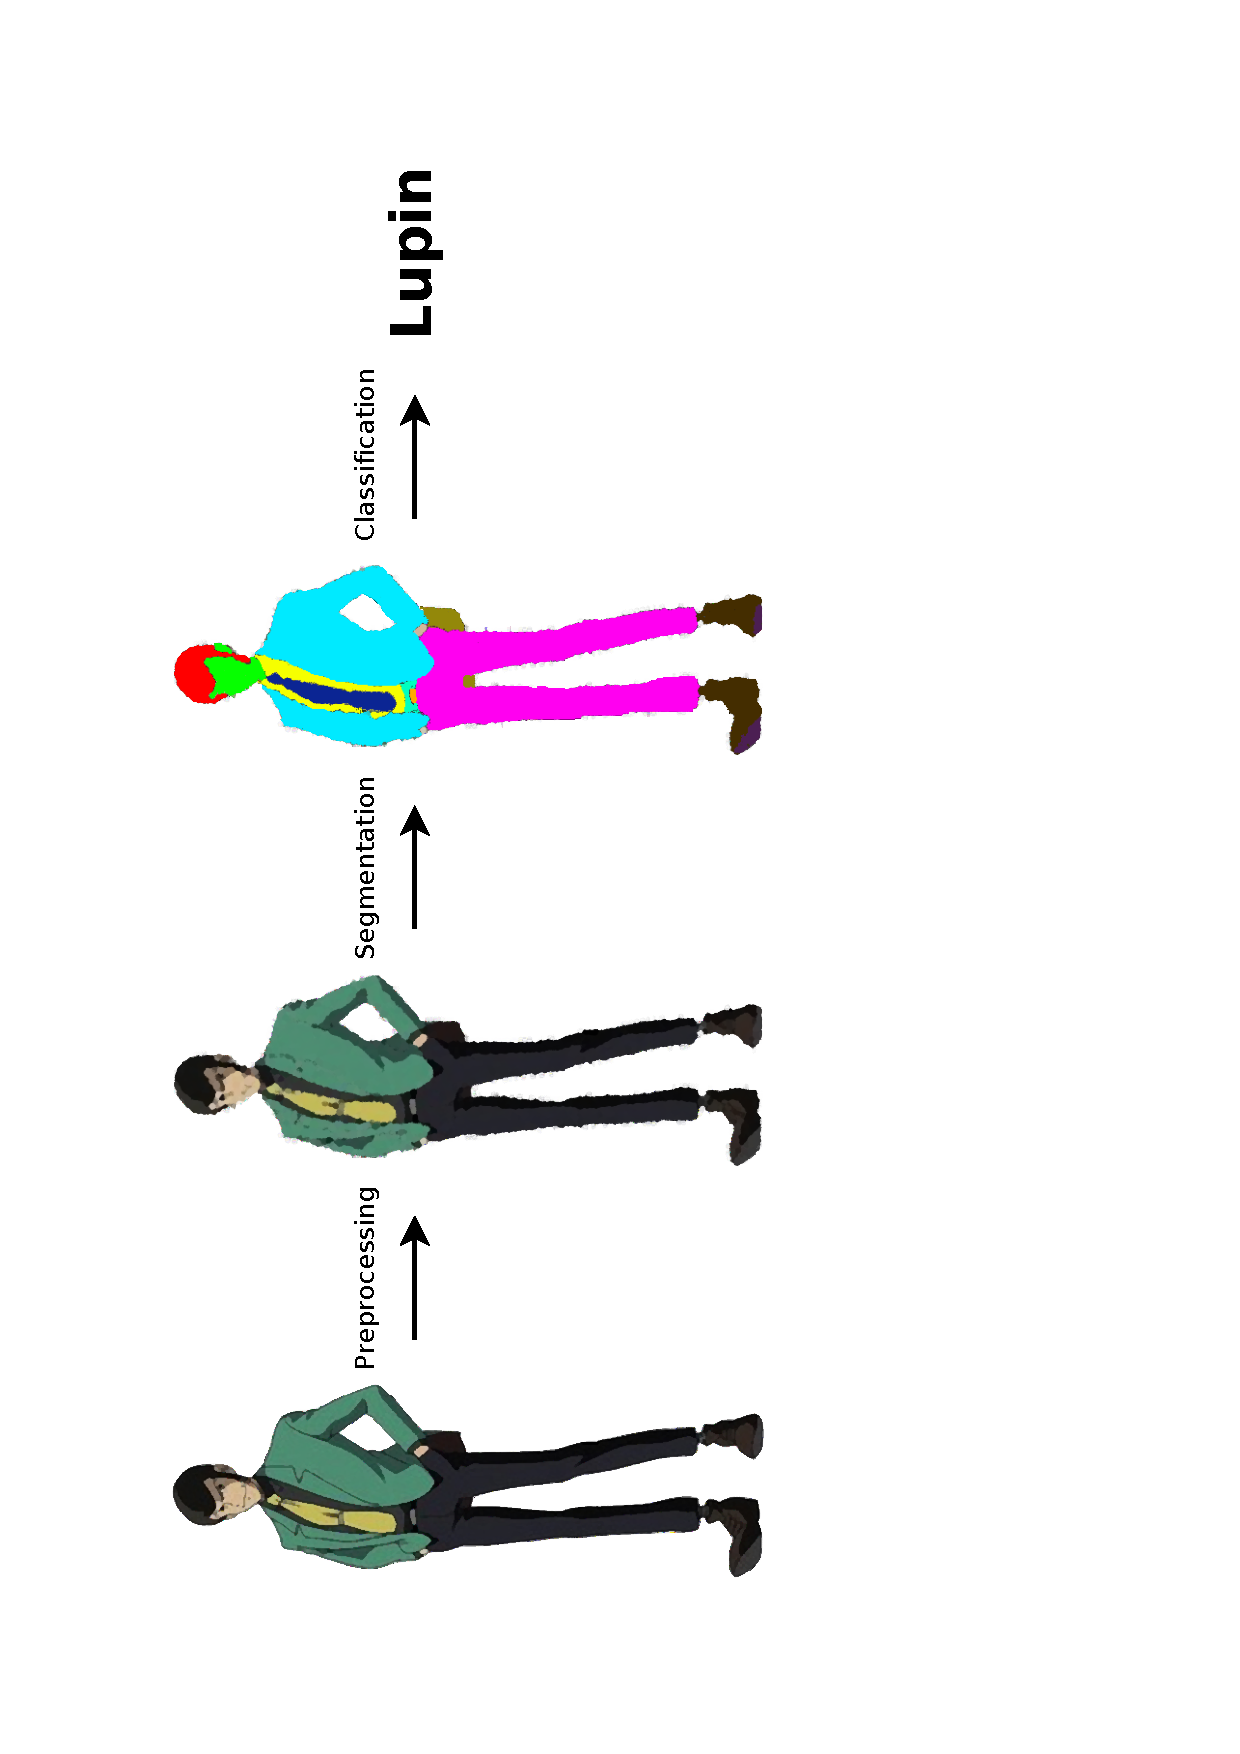
\includegraphics[height=\textwidth,angle=270,clip=true,trim=2cm 0 6cm 0]{../images/visionSystemDiagram.pdf}
}
\caption{Diagram depicting how preprocessing, segmentation and classification interact.}
\end{figure}

\end{frame}

\section{Kuwahara filtering}

\begin{frame}
\begin{itemize}
\item Consider $4$ square windows around the pixel to filter.
\item Compute mean color and variance in lightness (L in HSL) for each window.
\item Assign mean corresponding to smallest variance.
\end{itemize}

\begin{figure}[htb!]
\centering
\begin{subfigure}{.24\textwidth}

\includegraphics[width=\textwidth]{../images/miku_d.png}
\caption{Before filtering.}
\end{subfigure}
\begin{subfigure}{.24\textwidth}

\includegraphics[width=\textwidth]{../images/miku_d_filtered_smallh.png}
\caption{Small window.}
\end{subfigure}
\begin{subfigure}{.24\textwidth}

\includegraphics[width=\textwidth]{../images/miku_d_filtered.png}
\caption{"good" window.}
\end{subfigure}
\begin{subfigure}{.24\textwidth}

\includegraphics[width=\textwidth]{../images/miku_d_filtered_largeh.png}
\caption{Large window.}
\end{subfigure}
\caption{Results of Kuwahara filtering with varying window size.}
\label{fig:kuwaharaExample}
\end{figure}

\end{frame}

\section{Segmentation by Felzenszwalb's method}

\begin{frame}
\begin{itemize}
\item Graph method based on Kruskal's algorithm.
\item Efficient: $O(n\log(n))$ time with $4$-connected neighborhood.
\item Accurate: neither too "coarse" nor too "fine".
\item But depends on a scale parameter $k$ which controls the size of segments.
\end{itemize}

\begin{figure}[htb!]
\centering
\begin{subfigure}{.3\textwidth}

\includegraphics[width=\textwidth]{../images/rufy_d.png}
\caption{Original image}
\end{subfigure}
\begin{subfigure}{.3\textwidth}

\includegraphics[width=\textwidth]{../images/luffyK100.png}
\caption{$k = 100$.}
\label{fig:smallKSegmentation}
\end{subfigure}
\begin{subfigure}{.3\textwidth}

\includegraphics[width=\textwidth]{../images/luffyK1000.png}
\caption{$k = 1000$.}
\label{fig:largeKSegmentation}
\end{subfigure}
\end{figure}

\end{frame}

\begin{frame}
\begin{itemize}
\item Post processing by merging segments with close hue.
\item Allows varying segment sizes and non connected segments.
\end{itemize}

\begin{figure}[htb!]
\centering
\begin{subfigure}{0.3\textwidth}

\includegraphics[width=\textwidth]{../images/miku_a.png}
\caption{Original image.}
\end{subfigure}
\begin{subfigure}{0.3\textwidth}
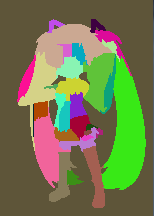
\includegraphics[width=\textwidth]{../images/miku_seg_initial.png}
\caption{Before merging.}
\end{subfigure}
\begin{subfigure}{0.3\textwidth}
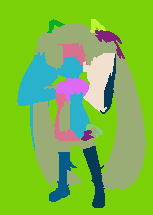
\includegraphics[width=\textwidth]{../images/miku_seg_fused.png}
\caption{After merging.}
\end{subfigure}
\end{figure}
\end{frame}

\section{Classification by spectral method}

\section{Classification by segment matching}

\section{Results and analysis}
\end{document}